\section*{The Discrete Fourier Transform}

\subsection*{The DFT Equation}

We now have all the necessary knowledge to understand how the Discrete Fourier Transform works.  In fact, we
have essentially walked through most of it during our discussion of orthogonality and the inner product.  Before
I present the equation, remember that the DFT takes a finite number of samples and produces a finite frequency
spectrum.  The DFT makes an important assumption about those samples: \textbf{the samples contain an integer number 
of periods from some periodic signal}.  If the signal is periodic, then we know it can be represented as a sum of
harmonic sinusoids.  Therefore, we only need to test our signal for the harmonics instead of the entire frequency
spectrum.  This is tremendously important because we need to generate a finite frequency spectrum.  Furthermore,
assuming we have filtered out any frequency components above the Nyquist frequency, we only need to test harmonics
up to the Nyquist frequency.  The fundamental frequency of the harmonics is simply the duration represented
by the samples.  


Here is the equation for the DFT below:

\begin{equation}
\label{eq:dft}
X_k = \sum_{n = 0}^{N - 1}x[n] \cdot e^{-i\frac{2\pi}{N}kn}
\end{equation}

There is a lot to unpack here.  At a high level $X_k$ represents how much of some frequency we have in
some signal $x[n]$.  $X_k$ is a complex number and is the result of the inner product of our signal $x[n]$
and some test frequency denoted by the complex exponential $e^{-i\frac{2\pi}{N}kn}$.  If $X_k$ is zero, then
we know we do not have that frequency in $x[n]$.  If $X_k$ is non-zero, then we do have some amount of 
that frequency in $x[n]$.  

The DFT equation is just a mathematical description of the procedure described 
in Figure \ref{fig:testComplex}.  Importantly, \textbf{the equation for the DFT tests only one frequency.}  
$X_k$ is the result of just one test.  To build the entire frequency spectrum for an audio signal, we would
need to use the DFT equation multiple times.

Noticeably absent though from Equation \ref{eq:dft} is any mention of frequency, usually described with the
variable $f$.  Understand that the DFT is in fact calculating the inner product of the signal $x[n]$ with some
 frequency.  However, we cannot determine the frequency without knowing the sampling rate.  This is
 true if we look at any sequence of samples including those operated on by the DFT.
Take a sequence of samples from a simple sine wave.  We actually cannot make any
claims about the frequency of that sinusoid.  We need to know how fast those samples will be played back.  
 The faster the playback, then the higher the frequency.  Similarly, the slower the playback, then the lower
 the frequency.  Frequency can only be determined by the combination 
 of a sequence of samples in conjunction with a sampling rate, usually notated as $f_s$.  With the DFT, we
 make no assumptions about the sampling rate of the signal $x[n]$.  We treat $x[n]$ as just a sequence of
 samples and we test every sinusoid that could be periodic along that sequence of samples.

Remember orthogonality for finite sinusoids only holds for periodic sinusoids.  A sinusoid is periodic if it
completes an integer number of cycles across some period. 
In the DFT, that period is the number of samples of our audio signal $x[n]$ denoted by $N$. 
The variable $k$ denotes
the number of complete cycles that our testing sinusoid completes and specifies a harmonic
to test against $x[n]$.  If we know the sample rate $f_s$, we
can determine the frequency of the sinusoid we are testing using $k$ and $N$.  The sample rate is a ratio of
the number of samples taken per second.  If we divide the sample rate by $N$, we can calculate how many 
periods of $N$ it takes to span one second of time.  For example if $f_s = 1000$Hz and $N = 250$, then
$f_s/N = 4$ tells us that four cycles of $N$ constitutes one second of time.  If we know that our testing sinusoid
completes $k$ cycles over those $N$ samples, then it must complete $k \cdot f_s/N$ cycles per second.  This is
the frequency of the testing sinusoid.  Therefore, we can state that 

\begin{equation}
	\label{eq:freq}
	f = \frac{k}{N}f_s
\end{equation} 

\noindent Once we have the sampling rate, we know the
frequency represented by $X_k$.  In fact, you can see in the complex sinusoid
all the components for determing frequency (i.e., $\frac{k}{N}$) except the sampling rate.  
	
	Perhaps
you may be wondering why the sample rate is simply not included in the DFT equation.  That's a reasonable 
question and would make sense in the domain of audio.  In fact, we could write a variation of the DFT equation
that takes into account the sample rate of our signal by rearranging Equation \ref{eq:freq} and substituting it
into the DFT equation from Equation \ref{eq:dft}.

\begin{equation}
\label{eq:dftFS}
	X_f = \sum_{n = 0}^{N - 1}x[n] \cdot e^{-i2\pi \frac{f}{f_s}n}
\end{equation}

\noindent Here we take the same inner product of $x[n]$ with some complex sinusoid of frequency $f$ and known sample
rate $f_s$.  It is easy to see that this new variation is equivalent to Equation \ref{eq:dft} by the fact that 
$f = \frac{k}{N}f_s$.  However, if you were to use the version of the DFT from Equation \ref{eq:dftFS}, you
would need to be sure that the frequencies you tested were in fact periodic along the interval $N$.  While Equation
\ref{eq:dftFS} may translate the standard DFT equation to the variables of $f$ and $f_s$ with which you are likely
more comfortable, it becomes much less obvious what frequencies actually do complete an integer number
of cycles along $N$.  That is the purpose of the variable $k$ and why Equation \ref{eq:dft} is actually the easier
way to view the computation of the DFT.  It is also very little work to figure out the frequency with 
$f = \frac{k}{N}f_s$.

Below summarizes the meaning of each variable in the DFT equation.

\begin{itemize}
	\item $x[n]$: the signal
	\item $n$: the indexing variable
	\item $X_k$: a complex number that is the result of the inner product of $x[n]$ and a complex sinusoid
	\item $k$: the number of complete cycles our testing complex sinusoid completes
	\item $N$: the number of samples of our signal $x[n]$
	\item Frequency can be determined if the sampling rate is known by using $f = \frac{k}{N}f_s$
\end{itemize}

\subsection*{A Simple Example}

Let us use a simple example to illustrate the DFT equation.  Suppose
we have samples drawn from the following signal $x = 0.5\cos(2\pi t + \pi) + 0.25\cos(4\pi t - 1)$.  The signal
$x$ contains two sinusoids of frequency 1Hz and 2Hz, respectively, with differing phases and amplitudes.  
Let us say we
were to draw eight samples ($N = 8$) from $x$ at a sampling rate of 8Hz for ease.  Here are those samples below:

$$x[n] = [-0.3649, -0.1432, -0.1351, 0.1432, 0.6351, 0.5639, -0.1351, -0.5639]$$

Now let us use the DFT equation to check whether $x[n]$ contains the frequency 2Hz.  We 
of course know that it does but let us ensure that the DFT returns a non-zero value.  We
need to first figure out what $k$ should be.  We can simply solve using $f = \frac{k}{N}f_s$ and determine that
for $f = 2$, we should use $k = 2$.  Plugging in our values for $k$ and $N$ into Equation \ref{eq:dft}, we now 
need to compute the following:

$$X_2 = \sum_{n = 0}^{7}x[n] \cdot e^{-i\frac{\pi}{2}n}$$

\noindent Unfortunately, we cannot just simply plug this into our normal calculators and figure out what $X_2$ is.  The complex exponential needs to be converted into its sinusoidal form using Euler's formula as shown in Equation
 \ref{eq:euler}.  So let us rewrite that now:

$$X_2 = \sum_{n = 0}^{7}x[n] \cdot (\cos{(-\frac{\pi}{2}n)} +  i\sin(-\frac{\pi}{2}n)) = 
\sum_{n = 0}^{7}x[n]\cos{(-\frac{\pi}{2}n)} + i\sum_{n = 0}^{7}x[n]\sin(-\frac{\pi}{2}n))$$

\noindent Let us calculate each summation independently.  The left summation is the real part of the complex number $X_2$
and the right summation is the imaginary part.  

\begin{align*}
	\sum_{n = 0}^{7}x[n]\cos{(-\frac{\pi}{2}n)} =  & (x[0] \cdot 1) + (x[1] \cdot 0) + (x[2] \cdot -1) + (x[3] \cdot 0)\\
	& + (x[4] \cdot 1) + (x[5] \cdot 0) + (x[6] \cdot -1) + (x[7] \cdot 0)\\
	=  & x[0] - x[2] + x[4] - x[6] \\
	=  & -0.3649 - (-0.1351) + 0.6351 - (-0.1351) \\
	= & 0.5404
\end{align*}

Half of the result trivially goes away because many of those samples are multiplied by zero.  The bracket notation
$x[1]$, for example, simply means to use the first sample from $x[n]$.  Note that we count starting from index zero
in this notation so $x[1] = -0.1432$ and not $-0.3649$.  Using the same procedure, we can calculate
the imaginary summation as well.  That result is $-0.8415i$.  Therefore, the value of 
$X_2$ is $0.5404 - 0.8415i$.  Note that $X_2$ is non-zero!  Therefore we can see that the frequency 2Hz is
indeed part of our signal as it should be.

If we want to test whether 3Hz is a part of $x[n]$, then we can calculate the DFT with the appropriate $k$ for
3Hz which also happens to be 3.  Using the same procedure, we would find that $X_3 = 0 + 0i$.  $X_3$ is
zero, meaning that 3Hz is not part of $x[n]$ as expected.  Of course, we will almost always be using the
DFT on unknown signals for $x[n]$.  But as this small example illustrates, the DFT can let us test to see 
whether a periodic sinusoid is part of our periodic signal.

\subsection*{Reconstructing Amplitude and Phase}

While the DFT can tell us whether a certain frequency is part of some signal, it can do even better.  The complex
number $X_k$ can be used to reconstruct the amplitude and phase of the frequency as well.  Let us assume that
$x[n] = A\cos(2\pi f Tn + \phi)$ and that $x[n]$ is periodic along the interval
 $N$.\footnote{We could very well assumed a sinusoid of the form $A\sin(2\pi fTN + \phi)$ instead of using a 
cosine.  It certainly makes no mathematical difference as a sine wave and cosine wave are only differentiated
by their phase.  It will be nicer mathematically if we think about it as a cosine wave.  The corresponding
$X_k$ would have a complex number of the form $	X_k = \frac{AN\sin(\phi)}{2} - \frac{AN\cos(\phi)}{2}i$. While this is perfectly valid, the careful reader will note that the angle or argument of the complex number
does not match $\phi$ as it does in the cosine form.  The cosine form presents a nice convenience.}  
Therefore, we can also write the sinusoid in the form $A\cos(2 \pi \frac{k}{N} n + \phi)$ using Equation \ref{eq:freq}.  The
latter form matches nicely with $X_k$ because the subscript $k$ from $X_k$ is the same $k$ in 
$A\cos(2 \pi \frac{k}{N} n + \phi)$.  When we take the DFT for $x[n]$,  the complex number will be of the form
shown in Equation \ref{eq:complexNumber}.

\begin{equation}
	\label{eq:complexNumber}
	X_k = \frac{AN\cos(\phi)}{2} + \frac{AN\sin(\phi)}{2}i
\end{equation}

 In some notations for complex numbers, the real part and imaginary parts of a complex number are referred to
 using the following operators: $\RE()$ and $\IM()$, respectively.  If the imaginary number $z = 3 + 4i$, then
 $\RE(z) = 3$ and $\IM(z) = 4$.  The symbols themselve may seem cumbersome but they are
 simply a convenience for referring to the components of an imaginary number.  Therefore, we can say
 based on Equation \ref{eq:complexNumber} that $\RE(X_k) = \frac{AN\cos(\phi)}{2}$ and $\IM(X_k) = 
 \frac{AN\sin(\phi)}{2}$.  Given Equation \ref{eq:complexNumber} and our new notation, the amplitude $A$ 
 can be dervied from $X_k$ as follows:


\begin{equation}
\label{eq:amplitude}
	A = \frac{2}{N}\sqrt{(\RE(X_k))^2 + (\IM(X_k))^2}
\end{equation}

Recalling our example above, let us reconstruct the amplitude from $X_2 = 0.5404 - 0.8415i$.  Plug in 
the real and imaginary components to Equation \ref{eq:amplitude}.  We then get 
$A = \frac{2}{8}\sqrt{(0.5404)^2 + (-0.8415)^2} = 0.25$.  If we look back at the original signal $x =
0.5\cos(2\pi t + \pi) + 0.25\sin(4\pi t - 1)$, you will see that the sinusoid with frequency 2Hz does indeed
have an amplitude of 0.25.  For those familiar with complex numbers, Equation \ref{eq:amplitude} looks 
remarkably close to the formula for the magnitude of a complex number.  The magnitude of complex number
$z$ is $\sqrt{(\RE(z))^2 + (\IM(z))^2}$.  The only difference then is a scaling factor of $2/N$.  Equation \ref{eq:amplitude}
is sometimes referred to as the ``normalized magnitude".

Similarly, we can also use $X_k$ to reconstruct the phase $\phi$ of the sinusoid.  Equation \ref{eq:phase}
shows the formula for doing so.

\begin{equation}
\label{eq:phase}
\phi = \tan^{-1}\bigg(\frac{\IM{(X_k)}}{\RE{(X_k)}}\bigg)
\end{equation}

\noindent From the same example, if we compute $\tan^{-1}(\frac{-0.8415}{0.5404})$, we get $-1$ which is indeed the
phase of $0.25\sin(4\pi t - 1)$.  One needs to be careful when using the inverse tan function with computers
or calculators.  The sign of the real and imaginary part indicates which quadrant the phase will be located.  Most
computers and calculators however wrap the phase between $-\frac{\pi}{2}$ and $\frac{\pi}{2}$.  Some software
like Matlab and others offer a special function that accounts for the sign of the numerator and denominator.  It is sometimes referred to as ``atan2".  It is fine to use either but you may need to correct some phases by 
hand if your calculator wraps the phase between $-\frac{\pi}{2}$ and $\frac{\pi}{2}$.

Equations \ref{eq:complexNumber}, \ref{eq:amplitude}, and \ref{eq:phase} apply to nearly all $X_k$. 
The exceptions are when $k/N$
is a multiple of $\frac{1}{2}$, corresponding to $k = N/2$ (i.e., the Nyquist frequency) and $k = 0$ 
(sometimes termed the DC offset in electronics).\footnote{DC offset refers to how far away the average of a signal
deviates from zero.  It is not a component of the signal that contributes to pitch.}  In these 
instances, the complex number $X_k$ cannot be used to recover the original amplitude and phase because
$X_k = AN\cos{(\phi)} + 0i$.  Since the imaginary component is zero, we do not know
what proportion of $A$ and $\phi$ contribute to the real component of $X_k$.  For the DC offset, this is not an issue.
A sinusoid with $k = 0$ is simply of the form $A\cos(\phi)$ and evaluates to a scalar.  It does not matter
what proportion of amplitude and phase contribute to the scalar, simply the value of the scalar itself.  The
Nyquist frequency  similarly does not pose a problem.  We do not expect to have
any frequency component at the Nyquist frequency if we have properly filtered our signal to prevent aliasing.

\subsection*{Frequency Bins}

The DFT equation from Equation \ref{eq:dft} only calculates the inner product of $x[n]$ and one
frequency.  However, we want to calculate the DFT for numerous frequencies.  Remember that
frequency is not explicitly stated in the DFT equation but rather implied by $k$ in conjunction with the 
sampling rate.  To flesh out the full frequency spectrum, $X_k$ is calculated for every value of $k$ from 0  to $N - 1$. 
Each calculation of $X_k$ is sometimes referred to as a frequency bin. 
A value of $k = 0$
calculates how much DC offset is in the signal (i.e., if the averages of the samples is something other than zero).
A value of $k = \frac{N}{2}$ tests for presence of the Nyquist frequency defined as half the sampling rate.  We do
not need to test for values of $k \geq N$ because the values of the DFT repeat.
You can test this yourself as $X_0 = X_N$ and $X_1 = X_{N + 1}$ and so on.

\begin{figure}[h] 
	\caption{A table of the DFT results from samples of $0.5\cos(2\pi t + \pi) + 0.25\cos(4\pi t - 1)$}
	\label{fig:dftTable}
	\begin{center}
		\begin{tabular}{ |c|c|c|c|c|c|c| } 
			\hline
			k & Frequency (in Hz) & $X_k$ & Amplitude & Phase \\ 
			\hline
			0 & 0 & $0 + 0i$ & 0 & 0 \\ 
			1 & 1 & $-2 + 0i$ & 0.5 & $\pi$ \\
			2 & 2 & $0.5403 - 0.8415i$ &0.25 & -1 \\
			3 & 3 & $0 + 0i$& 0 & 0 \\
			4 & 4 & $0 + 0i$  & 0 & 0 \\
			5 & 5 & $0 + 0i$  & 0 & 0 \\
			6 & 6 & $0.5403 + 0.8145i$ & 0.25 & $1$ \\
			7 & 7 & $-2 + 0i$  & 0.5 & $-\pi$ \\
			\hline
		\end{tabular}
	\end{center}
	
\end{figure}

Figure \ref{fig:dftTable} shows a table of all the calculations from the DFT in the column labeled $X_k$.  For
convenience, the frequency of each bin is also given.  Because the number of samples equals the sampling rate,
$k$ is equivalent to frequency of the $k$th bin, but that will rarely be the case.  We generally deal with very high
sampling rates like 44.1kHz and smaller numbers of samples for the DFT.  To calculate the frequency of each
$X_k$, sometimes referred to as frequency bins, we simply compute $k\frac{f_s}{N}$.  You can see that in
our trivial example that $\frac{f_s}{N} = \frac{8}{8} = 1$ so the frequency of each bin is just $k$.

Figure \ref{fig:dftTable} also has  columns for amplitude and phase as calculated using Equations 
\ref{eq:amplitude} and \ref{eq:phase},
respectively.  We can see that for a frequency of 1Hz there exists
 a sinusoid of amplitude 0.5 and phase $\pi$ and for a frequency of 2Hz there exists a sinusoid of 
 amplitude 0.25 and phase $-1$.  As expected the samples for $x[n]$ were taken from a signal 
 matching the specifications of those two sinsusoids, namely $0.5\cos(2\pi t + \pi) + 0.25\cos(4\pi t - 1)$.
 
 We can also see that we seemingly have extra sinusoids in our frequency domain at 6Hz and 7Hz.  
 We can ignore these frequencies.  The DFT is symmetric about the Nyquist frequency so any 
 frequencies below the Nyquist frequency will appear above the Nyquist frequency.  This is simply
 a byproduct of the math used for the DFT.  We could have simply just calculated the frequency
 for bins $k = 0$ up to the Nyquist frequency.  However, the standard frequency domain computed
 by the DFT ranges from $k = 0$ to $N - 1$.  For audio signals, the upper half of the frequency
 domain is unimportant but for different signals it is.
 
\subsection*{Interpreting The Magnitude and Phase Spectra}

When we calculate the DFT,  we often display the magnitude and phase of each $X_k$ graphically.  Below
are two examples of the magnitude and phase spectrum of some signal $x[n]$ with sample rate $f_s = 256$Hz and
$N = 128$.  Let us see what we can deduce about the time domain form of the signal from these two spectrums.

\begin{figure}[h]
	\caption{The magnitude spectrum of $x[n]$ at $f_s = 256$ and $N = 128$}
	\label{fig:magnitudeGraph}
	\begin{center}
	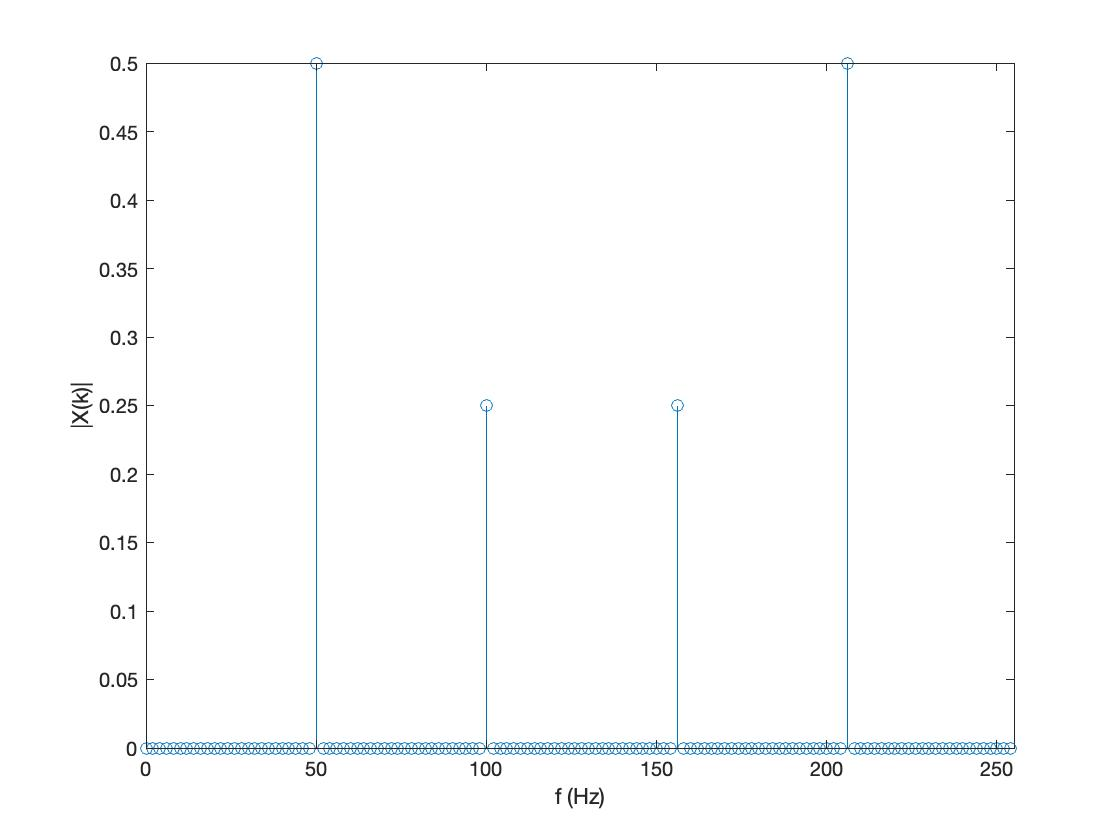
\includegraphics[scale = 0.3]{magnitude.jpg}
	\end{center}
\end{figure}

\begin{figure}[h]
	\caption{The phase spectrum of $x[n]$ at $f_s = 256$ and $N = 128$}
	\label{fig:phaseGraph}
	\begin{center}
		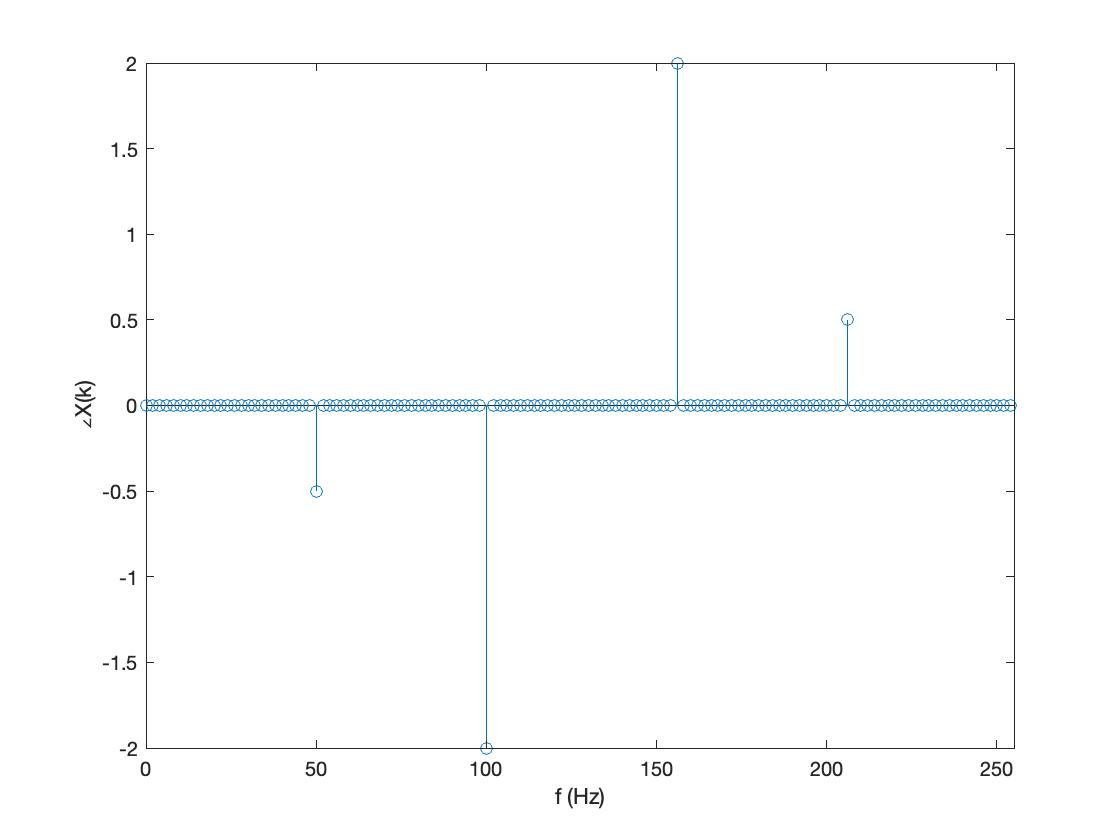
\includegraphics[scale = 0.3]{phase.jpg}
	\end{center}
\end{figure}

Figure \ref{fig:magnitudeGraph} shows the magnitude spectrum of $x[n]$.  Here we plot the magnitude of
each $X_k$.  Recall that the magnitude of a complex number $z$ is defined as $\sqrt{(\RE(z))^2 + (\IM(z))^2}$.
It is quite common to see plots of the magnitude spectrum
using simply the magnitude of each $X_k$.  To derive the amplitude of the original frequencies, we must multiply
each value in the figure by $2/N$ to match Equation \ref{eq:amplitude}.  
Alternatively, some magnitude spectrum are plotted on a decibel scale.  It is always important to
check how the magnitude spectrum is plotted as there are several variations.

	In Figure \ref{fig:magnitudeGraph}, we see four peaks in the graph.  We can conclude that there are four 
frequency components at frequencies 50Hz, 100Hz, 156Hz, and 206Hz.  
We can ignore the components of the spectrum above the Nyquist frequency of 128Hz. 
Therefore, we have two
sinusoidal components in $x[n]$: 50Hz at an amplitude of 0.5 and 100Hz at an amplitude of 0.25.  

Note the symmetry in the magnitude spectrum.  If we were to draw a straight line down the center of the 
magnitude spectrum at the Nyquist frequency, the left half and right half would be perfectly symmetrical.  
A fundamental property of the DFT is that when $x[n]$ is a real signal and does not include any complex
components, the two halves of the magnitude spectrum are symmetrical.  Because we are dealing solely 
with audio signals,
we always use the DFT with real signals and therefore will always have symmetry.  

Figure \ref{fig:phaseGraph} shows the phase spectrum of $x[n]$.  The phase spectrum of a signal plots
the argument of the complex number $X_k$.  Those familiar with complex numbers will note that
 the argument of a complex number is also calculated 
using Equation \ref{eq:phase}.  Thus, the argument of each $X_k$ is the same as the phase of
the frequency component, assuming we model the frequency component 
as a cosine wave.  As expected we see peaks at exactly 50Hz, 100Hz, 156Hz, and 206Hz.  Again, we can 
ignore the two frequencies above the Nyquist frequency.  We can see phases of $-0.5$ and $-2$ at 50Hz and 
100Hz, respectively.  Putting together the information from the magnitude and
phase spectrum, we can perfectly recreate the original signal: 
$x[n] = 0.5\cos(2\pi(50)t - 0.5) + 0.25\cos(2\pi(100)t - 2)$.

There is also symmetry in the phase spectrum as well.  Again if we were to draw a straight line vertically at
the Nyquist frequency and flip the signs of one of the halves, we would have two symmetrical halves.  Again
these symmetrical properties are true for all real signals $x[n]$ such as audio.
